\subsection{UC 5: Gestione Progetti}
		\centering
		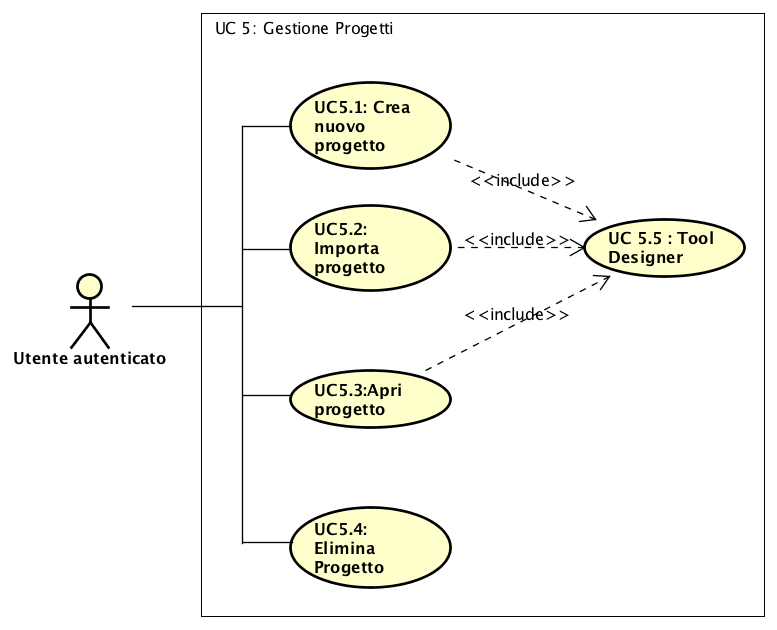
\includegraphics[scale=0.7]{../../Casi D'uso/UC5.png}
\begin{itemize}
		\item \textbf{Attori coinvolti:} Utente autenticato \\
		\item \textbf{Scopo e descrizione:} L'utente ha la possibilità di creare un nuovo progetto, modificare un progetto esistente, salvare un progetto o eliminare un progetto. \\
		\item \textbf{Precondizione:} L’applicazione visualizza i pulsanti predisposti per l’esecuzione di azioni sopra indicate. \\
		\item \textbf{Postcondizione:}L’applicazione, a seconda dell’azione scelta dall’utente, svolgerà le sue funzioni. \\
\end{itemize}